\section{Volume conductor theory}
\label{sec:VC}
\index{Volume conductor}

As we saw in the previous section, simulations of morphologically complex neurons allow us to compute the transmembrane currents entering/leaving the neuron at various locations. This chapter is about how we, when we know the distribution of neuronal current sources, can use volume conductor (VC) theory to predict the extracellular potential at a given point in space. VC theory is the fundament for forward modeling of extracellular potentials at different spatial scales, from extracellular spikes, LFPs and MUAs, to ECoGs and EEGs.

As used in neuroscience, VC theory rests on a set of assumptions regarding the nature of extracellular current densities ({\bf i}), the medium that they travel through, and the effective conductivity ($\sigma$) for an extracellular current. Instead of introducing these assumptions right away, we start with presenting the VC theory in the form in which it is most commonly used, and postpone a more thorough discussion of the underlying assumptions to the end of the chapter. Before we start deriving the theory, however, we need to make a note on how we approximate the extracellular medium, i.e., the medium that an extracellular current travels through.


%%%%%%%%%%%%%%%%%%%%%%%%%%%%%%%%
\subsection{\blue{Continuous, porous medium approximation for VC theory}}
\label{sec:continuous}
%%%%%%%%%%%%%%%%%%%%%%%%%%%%%%%%
When presenting the theory for modeling single neurons (Chapter \ref{sec:Neuron}), we may have given the impression that they are solitary creatures living in a vast extracellular space with long distances to their nearest cell neighbors. This is far from the truth. A cross section of a piece of brain tissue shows that it is densely packed with neural and glial processes (Fig.\ref{VC:fig:ECS}). The extracellular space (colored red in the figure) occupies only about 20 \% of the the total tissue volume. Moreover, it has a highly tortuous geometry, with an average intercell-distance of about 40-60 nm \citep{Sykova2008}. 

\begin{figure}[!ht]
\begin{center}
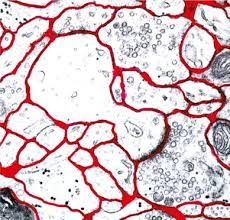
\includegraphics[width=0.3\textwidth]{Figures/VC/ECSdummy.jpeg}
\end{center}
\caption{\textbf{Tortuous medium}  Cross section image of a piece of neural tissue. Extracellular space (marked red) occupies about 20 \% of the total tissue volume, and has a highly tortuous structure. Placeholder, taken from \cite{Sykova2008}.
\tvnnote{Vi får vel lage vår egen illustrasjon her, kanskje med panel A lik denne, og panel B en zoomet ut versjon der det ser mer homogent ut?}
}
\label{VC:fig:ECS}
\end{figure}

At the microscopic scale, the conductivity $\sigma$ in the brain tissue is thus highly non-homogeneous. For example, it will be very high at a cellular membrane and much lower in the extracellular space between membranes. Accordingly, electric potentials can vary greatly over tiny distances, and become very large near cell membranes. When we study extracellular potentials, we are typically not interested in these microscopic variations in $\sigma$ and $\phi$, but rather in the values of these entities when averaged over some spatial volume. In practice, the electrodes used in experimental recordings perform such an averaging. Sizes of electrodes used to record extracellular potentials typically range from 5 $\mu$m to 125 $\mu$m in diameter\cite{Viswam2019}, which is larger than the typical diameter of a dendrite ($\sim$ 1 $\mu$m). Experimental recordings thus give us the average potential over a region in space that typically spans over both extracellular space and several neural and glial processes. It is thus the dynamics at this coarse grained spatial scale that we will focus on.

At the coarse grained spatial scale, it is reasonable to assume that microscale inhomogeneities average out, and that the brain tissue can be treated as a continuous medium \cite{Gratiy2017}. The VC theory presented in this Chapter is based on the continuous medium approximation, and thus describes the extracellular dynamics on a coarse grained spatial scale, with a spatial resolution larger than a micrometer. 

A continuous, porous medium is defined by two key parameters \cite{Nicholson1981}. The first parameter is $\alpha$, is the fraction of the tissue volume that is extracellular space. It typically is about 0.2 in brain tissue, although this can vary between brain regions and even locally due to cellular swelling. The second parameter is $\lambda$, the tortuosity of the medium \cite{Nicholson1981}. It interprets as the ratio between the shortest pathway between two points in space and the euclidian distance between these two points. The tortuosity can be measured experimentally, and for extracellular transport, it has been found that $\lambda = 1.6$ \cite{Nicholson1998}. 

The continuous, tortuous medium approximation has implications for how we interpret the various concepts and variables that we use, so we here give a brief list of definitions: 

\begin{itemize}
\item We will use the term "extracellular medium" to refer to the tissue as it is \textit{experienced} by extracellular currents. It is not the same as the "extracellular solution", i.e. the fluid filling the extracellular space. The extracellular medium is a medium where extracellular currents (i) are confined to move predominantly through the fraction $\alpha$ of the total medium volume, and (ii) must take detours around neural and glial obstacles, as reflected through the tortuosity $\lambda$ \citep{Nicholson1998, Nunez2006}. 

\item  {\bf i} (units $\mathrm{A/m^2}$) will denote the current density for currents traveling extracellularly through the brain tissue. It is defined as current per unit \textit{tissue} (cross-section) area.

\item $\phi$ (unit V) will be used to denote the extracellular potential on the coarse grained scale, i.e., it will represent the extracellular potential averaged over some volume of at least a cube micrometer.

\item $\sigma$ (units S/m) will denote tissue averaged extracellular conductivity, i.e., it is not the (microscopic) conductivity of the extracellular solution, but the coarse-grained conductivity of the extracellular medium as defined above, where the reduced volume fraction and tortuosity are accounted for. Experimental recordings of the extracellular conductivity typically measure 
$\sigma$ as defined in this way. For comparison, the microscopic and unhindered conductivity of the (pure) extracellular solution should theoretically be a fraction $\lambda^2/\alpha$ higher. 

\item $C$ (units A/m$^3$) will denote the current source density (CSD), defined as the local neuronal output current per unit tissue volume.

\end{itemize}

The continuous, porous medium approximation is revisited in Chapter \ref{sec:conductivity}, where we review experimental measurements and theoretical interpretations of the tissue conductivity.


%%%%%%%%%%%%%%%%%%%%%%%%%%%%%%%%
\subsection{\blue{From neuronal current sources to extracellular potentials}}
\label{sec:continuous}
%%%%%%%%%%%%%%%%%%%%%%%%%%%%%%%%
Throughout this chapter we shall assume that we know the neuronal (and glial) transmembrane currents at all points in space. If they stem from a simulation of a multicompartmental neuron model, they are typically represented as a set of discrete current sources, i.e., one source per neuronal segment (Fig. \ref{VC:fig:CSD}A). As a mathematical generality, we may instead define a continuous density distribution of current sources (Fig. \ref{VC:fig:CSD}B), which we call the current source density ($CSD$). For example, the $CSD$ representing the four point sources in Fig. \ref{VC:fig:CSD}A would be formulated as a sum of four delta functions. 

\begin{figure}[!ht]
\begin{center}
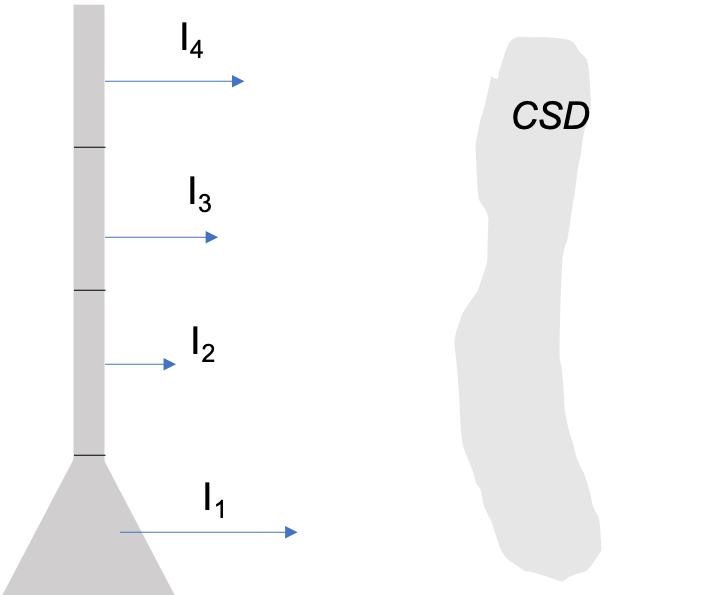
\includegraphics[width=0.3\textwidth]{Figures/VC/CSD.png}
\end{center}
\caption{\textbf{Neuronal current sources.}  {\bf (A)} When simulated on a numerical scheme, the transmembrane currents are known at a discrete set of neuronal segments, i.e., as a set of point sources.  {\bf (B)} As a mathematical generality, we can describe the transmembrane currents as a current source density (CSD) distribution, $C({\bf r},t)$. We note the sum of current entering/leaving a neuron is always zero, so that in {\bf (A)}, we must have that $I_1 + I_2 + I_3 + I_4 = 0$, and in {\bf (B)} we have that the spatial integral over $C$ must be zero.
}
\label{VC:fig:CSD}
\end{figure}
Volume conductor theory is essentially based on current continuity in the extracellular medium, i.e., the requirement that no net current can enter/leave a given point in space. Mathematically, current continuity implies that:
\begin{equation}
\nabla \cdot {\bf i}({\bf r}, t) = - C({\bf r}, t),
\label{eq:CSD1}
\end{equation}
where ${\bf i}$ is the extracellular current density, and $C$ is the current source density. What Eq. \ref{eq:CSD1} essentially tells us, is that if a neuron outputs a current into a (infinitesimal) volume of space (the $C$ term), an equally large current leaves that volume as an extracellular current (the $\nabla \cdot {\bf i}$ term).

In this chapter, we shall assume that the extracellular current density is described by:
\begin{equation}
{\bf i}({\bf r}, t) = - \sigma({\bf r}, t) \nabla \phi({\bf r}, t),
\label{eq:ohmici}
\end{equation}
where $\sigma$ is the effective conductivity for an extracellular current in brain tissue. If we combine Eq. \ref{eq:ohmici} and Eq. \ref{eq:CSD1}, we get:

\begin{equation}
\nabla \left( \sigma({\bf r}, t) \nabla \phi({\bf r}, t) \right) = - C({\bf r}, t),
\label{eq:CSD2}
\end{equation}

which simplifies to the more commonly used relation:
\begin{equation}
\sigma \nabla^2\phi({\bf r}, t) = - C({\bf r}, t),
\label{eq:CSD3}
\end{equation}
in the less general case where the conductivity $\sigma$ is constant. Hence, if we know the distribution of neuronal current sources, we can integrate eq. \ref{eq:CSD2} or eq. \ref{eq:CSD3} to predict the electrical potential in the extracellular space surrounding the sources. 

As indicated above, the variables ${\bf i}$, $\sigma$ and $\phi$ can in general be functions of both position and time. However, for the remainder of this chapter, we shall mostly assume that $\sigma$ is constant. Furthermore, it is implicit in eq. \ref{eq:CSD2} that the relationship between current sources and extracellular potentials is instantaneous (i.e., we can solve eq.  \ref{eq:CSD2} at each time point independently), and in the remainder of the chapter we therefore only use the positional argument for ${\bf i}$ and $\phi$. 

In the following subsections, we show how VC-theory is used to compute $\phi$ in some idealized cases with a homogeneous extracellular medium, and then discuss how this theory can be expanded to more complex cases accounting for inhomogeneities. 


%%%%%%%%%%%%%%%%%%%%%%%%%%%%%%%%
\subsection{\blue{Infinite isotropic homogeneous extracellular medium}}
\label{sec:isohomo}
%%%%%%%%%%%%%%%%%%%%%%%%%%%%%%%%
We shall now derive an expression for the extracellular potential $\phi$ in the case where the extracellular medium is infinite, isotropic and homogeneous. By homogeneous we mean that the conductivity $\sigma$ is the same everywhere in space, and by isotropic we mean that $\sigma$ is the same in all spatial directions. Although the extracellular medium in reality is neither infinite, nor strictly isotropic and homogeneous, this approximation may still in many cases give fairly good predictions of $\phi$.


%%%%%%%%%%%%%%%%%%%%%%%%%%%%%%%%
\subsubsection{\blue{Point source approximation}}
%%%%%%%%%%%%%%%%%%%%%%%%%%%%%%%%
We start by deriving the contribution to $\phi$ from a single neuronal point source $I_k$ at the point ${\bf r_k}=0$ (Fig. \ref{VC:fig:pointsource}A). 

\begin{figure}[!ht]
\begin{center}
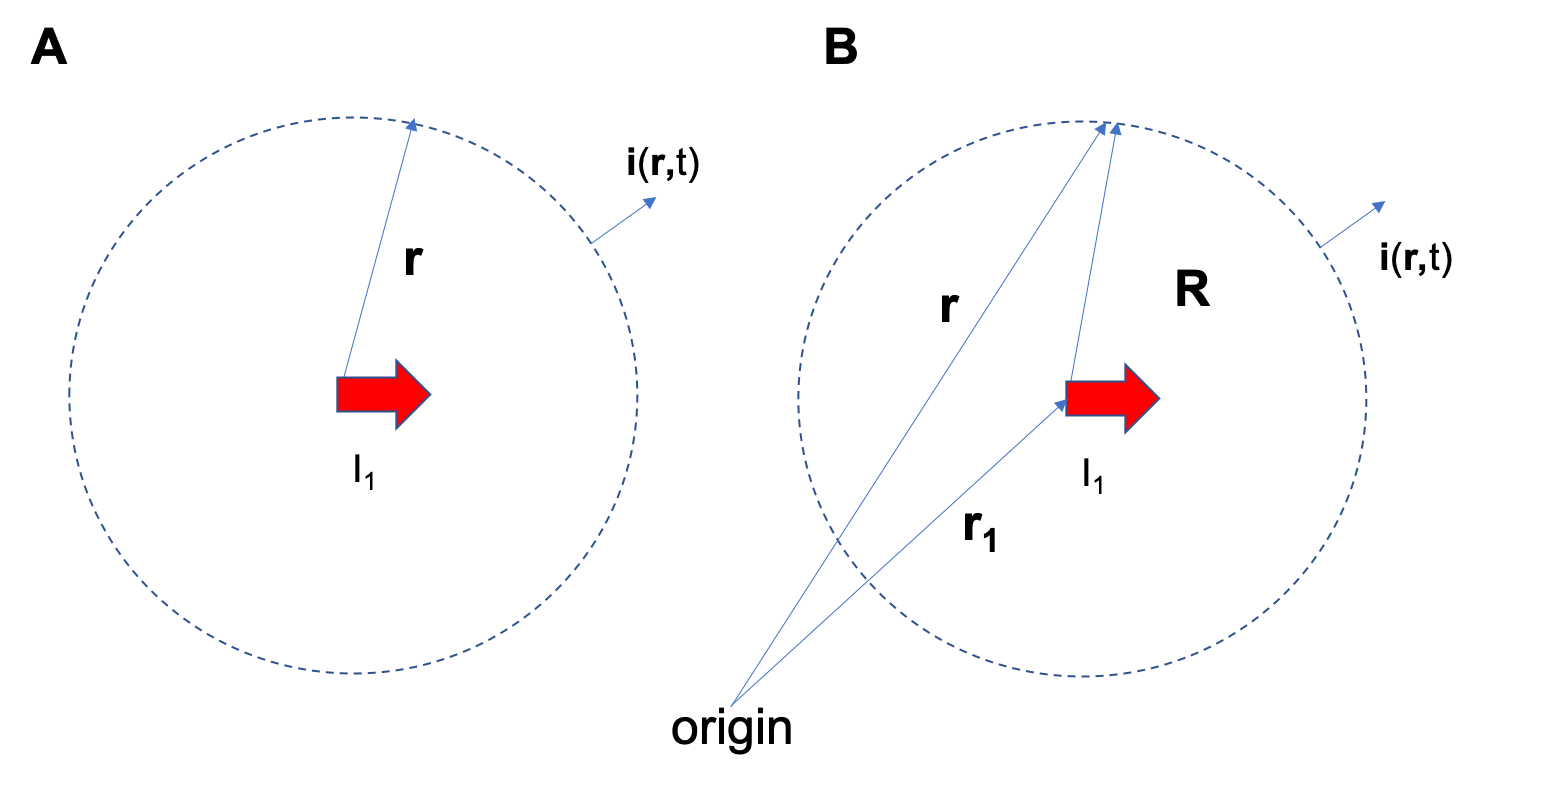
\includegraphics[width=0.6\textwidth]{Figures/VC/Pointsource.png}
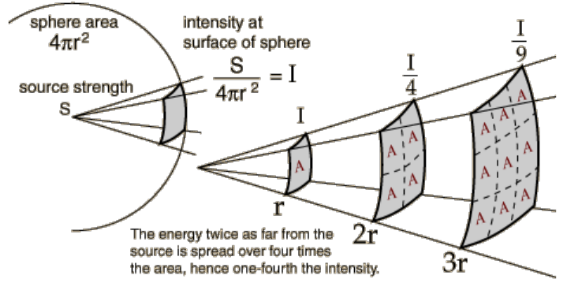
\includegraphics[width=0.6\textwidth]{Figures/VC/pointsource_3D_illustration.png}
\end{center}
\caption{\textbf{Extracellular field from single neuronal point source.} 
\tvnnote{Lage 3D versjon, inspirert av den underste?}
}
\label{VC:fig:pointsource}
\end{figure}

Here, we could compute $\phi$ by solving eq. \ref{eq:CSD3}. However, due to the spherical symmetry of this simple case, we can take a shorter path by realizing that the current density (eq. \ref{eq:ohmici}) must radially directed, and that its magnitude must be solely a function of distance $r$ from the source:

\begin{equation}
i({\bf r}) = i(r) = -\sigma \frac{d\phi(r)}{dr}.
\end{equation}

Knowing this, we may find $\phi$ by simply demanding that net current $I_k$ injected into the center of the spherical volume with radius $r$ must equal the net current leaving through the surface of the volume, which in turn must equal the current density $i(r)$ at the surface multiplied with the surface area $4\pi r^2$. We then get the relationship:

\begin{equation}
I_k = -4\pi \sigma r^2  \frac{d\phi(r)}{dr} \, \iff \, \frac{d\phi(r)}{dr} = -\frac{I_k}{4\pi \sigma r^2 }.
\label{eq:knut}
\end{equation}

To obtain the final solution for $\phi$, we integrate eq. \ref{eq:knut} from $r$ to $\infty$:

\begin{equation}
\int_r^{\infty} \frac{d\phi(r')}{dr'} dr' = \int_r^{\infty} -\frac{I_k}{4\pi \sigma r'^2 } dr'.
\label{eq:knut2}
\end{equation}
Since $\phi({\infty}) = 0$, this leads to the final expression:

\begin{equation}
\phi({\bf r}) = \phi(r) = \frac{I_k}{4\pi \sigma r},
\label{eq:pointsource}
\end{equation}
where $r$ is the distance from the source.

In the above, we made things simple by assuming that the current source was placed in the origin ${\bf r} = 0$. For a point source located in an arbitrary point ${\bf r_k} $, the corresponding expression for the extracellular potential is:

\begin{equation}
\phi({\bf r}) = \frac{I_k}{4\pi \sigma |{\bf r-r_k}|},
\label{eq:pointsource2}
\end{equation}

If we have several point-current sources, $I_{1}, I_2, I_3, ... $ in locations ${\bf r_1}, {\bf r_2}, {\bf r_3} ... $), their contributions add up linearly, and the potential in a point ${\bf r}$ is given by:

\begin{equation}
\phi({\bf r}) = \frac{I_1}{4\pi  \sigma {\bf |r-r_1|}} + \frac{I_2}{4\pi  \sigma {\bf |r-r_2|} } + \frac{I_3}{4\pi  \sigma {\bf |r-r_3|} } + ... = \sum_k \frac{I_k}{4\pi  \sigma {\bf |r-r_k|} }.
\label{eq:pointsources}
\end{equation}


%%%%%%%%%%%%%%%%%%%%%%%%%%%%%%%%
\subsubsection{\blue{Line source approximation}}
%%%%%%%%%%%%%%%%%%%%%%%%%%%%%%%%
Eq.~\ref{eq:pointsources} is referred to as the point-source approximation \citep{Holt1999, Pettersen2008a}, since it approximates the neuron as a set of point current sources, i.e., the neuron delivers to the extracellular space a singular current source per neuronal segment, located in the segment midpoint. 

A more sophisticated choice may be to assume that the transmembrane current is evenly distributed over the segment axis, a choice which is referred to as the line-source approximation \citep{Holt1999, Linden2014}. The contribution to the extracellular potential from a current $I_k$ in a segment $k$ can be found analytically by integrating eq. \ref{eq:pointsource} over the center-line axis of the compartment (see Appendix C in \citep{holt1998}). We here skip the derivation, but give the final solution. For a segment with length $\Delta s_k$, the contribution to the extracellular potential will be:

\begin{equation}
\phi({\bf r},t)_k = \frac{I_k}{4\pi \sigma} \int \frac{dr_k}{|{\bf r-r_k}|} = 
\frac{I_k}{4\pi \sigma \Delta s_k} \log \left| \frac{\sqrt{h_k^2+\rho_k^2}-h_k}{\sqrt{\ell_k^2+\rho_k^2}-\ell_k} \right|,
\label{eq:linesource}
\end{equation}
\tvnnote{How  about dropping the subscript k?}
\ghnote{Beholdt den pga bedre kommunikasjon m/ neste uttrykk}
Here $\rho_k$ is the distance perpendicular to the line segment, $h_k$ is the longitudinal distance from the end of the segment, and $\ell_k = \delta s_k + h_k$ is the longitudinal distance from the start of the segment (Fig.~\ref{VC:fig:line_source_illustration}). Eq. \ref{eq:linesource} and Eq. \ref{eq:pointsource} are the equivalent expressions where the transmembrane currents in a single neuronal segment are treated as a line source and point source, respectively. As for the point-source approximation, the contributions from several line-sources add up linearly. That is, if we have multiple segments $k$, the extracellular potential can be computed as:
\begin{figure}[!ht]
\begin{center}
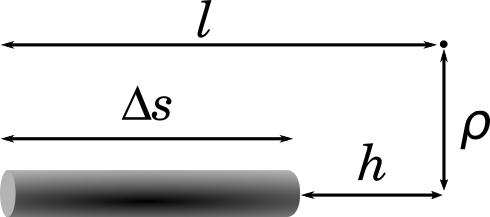
\includegraphics[width=0.4\textwidth]{Figures/VC/line_source_illustration.png}
\end{center}
\caption{\textbf{Line-source approximation.} 
\cite{Holt1998} \tvnnote{Add subscripts?}
}
\label{VC:fig:line_source_illustration}
\end{figure}

\begin{equation}
\phi({\bf r},{\bf t}) = \sum_k \frac{I_k}{4\pi \sigma \Delta s_k} \log \left| \frac{\sqrt{h_k^2+\rho_k^2}-h_k}{\sqrt{\ell_k^2+\rho_k^2}-\ell_k} \right|,
\label{eq:linesources}
\end{equation}

The line-source approximation is believed to give a better prediction of $\phi$ than the point-source approximation at points in space that are very near neuronal membranes, especially when it comes to predicting rapid fluctuations in $\phi$, such as the extracellular action potential signature \citep{Holt1999}. At points further away from membranes, the two approaches give converging predictions.


%%%%%%%%%%%%%%%%%%%%%%%%%%%%%%%%
\subsubsection{\blue{Current-source-density description}}
%%%%%%%%%%%%%%%%%%%%%%%%%%%%%%%%
The forward modelling formulas in Eq. \ref{eq:pointsources} and \label{eq:linesources} can be expressed more generally in terms of the CSD. The starting point is then eq. \ref{eq:CSD3}, which for a homogeneous and isotopic medium can be written: 

\begin{equation}
\nabla^2 \phi({\bf r}) = - \frac{C({\bf r})}{\sigma}
\label{eq:CSD4}
\end{equation}

Since this is a linear differential equation, we may solve it by first finding its Green's function, i.e., the solution to an impulse response $C({\bf r}) = I' \delta^3({\bf r-r'})$, where $\delta^3({\bf r})$ is the Dirac delta function in three dimensions, and $I'$ is the current source at this location. The general solution can then be expressed as a convolution over such Green's functions. Thus, we first seek the solution to: 

\begin{equation}
\nabla^2 \phi({\bf r}) = - \frac{I' \delta^3({\bf r-r'})}{\sigma}.
\label{eq:CSD5}
\end{equation}

We already listed the solution to this in eq. \ref{eq:pointsource2}, but we here provide a more rigorous derivation. We start by by integrating both sides of eq. \ref{eq:CSD5} over an arbitrary 3D volume containing the source:

\begin{equation}
\iiint_V \nabla^2\phi({\bf r}) \,dV =  - \frac{I'}{\sigma} \iiint_V \ \delta^3({\bf r-r'}) \, dV,
\label{eq:marit}
\end{equation}

By the definition of the delta-function, the right hand side of equation \ref{eq:marit} is simply $I'/\sigma$. Using Gauss' theorem, we can convert the volume integral on the left hand side of eq. \ref{eq:marit} to a surface integral, so that eq. \ref{eq:marit} becomes:

\begin{equation}
\oiint_{S} \nabla\phi({\bf r}) \cdot \, d{\bf S}  = - \frac{I'}{\sigma},
\label{eq:berit1}
\end{equation}

To solve this, it is convenient to chose the volume that we integrate over to be a sphere centered at the source location ${\bf r'}$, and with radius $R = |{\bf r-r'}|$ (Fig. \ref{VC:fig:pointsource}B). Due to the symmetry of problem, we then know that the electrical potential is the same for all ${\bf r}$ on the surface of the sphere, so that $\phi({\bf r}) = \phi(R)$. We also know that its gradient $\nabla\phi({\bf r}) = d\phi(R)/dR$ is constant over the surface, and perpendicular to the surface increment $d{\bf S}$. If we use this, eq. \ref{eq:berit1} becomes:
\begin{equation}
\oiint_{S} \frac{d\phi(R)}{dR} d{S}  = - \frac{I'}{\sigma},
\label{eq:berit1ogenhalv}
\end{equation}
which has the solution:
\begin{equation}
4\pi R^2 \frac{d\phi(R)}{dR} = \frac{I'}{\sigma}
\label{eq:berit2}
\end{equation}
If we integrate this from $R$ to $\infty$, and use that $\phi(\infty) = 0$, we get:
\begin{equation}
\phi(R) = \phi({\bf r}) = \frac{I'}{4\pi \sigma R}.
\label{eq:berit3}
\end{equation}
We may now insert back for $\phi(R)= \phi({\bf r})$ and $R = |{\bf r-r'}|$ to obtain the desired Green's function:

\begin{equation}
\phi({\bf r})= \frac{I'}{4\pi \sigma |{\bf r-r'}|},
\label{eq:berit4}
\end{equation}
As earlier stated, the solution for a general CSD can be expressed as a convolution over the Green's function, so that:

\begin{equation}
\phi({\bf r}) = \frac{1}{4\pi \sigma}\iiint_V \frac{C({\bf r'})}{|{\bf r}-{\bf r'}|} \,dV, 
\label{eq:csds}
\end{equation}
where the volume integral runs over all sources. Here, $C$ represents whatever approximation one used for the current sources, and eq. \ref{eq:csds} is the continuous counterpart to eq. \ref{eq:pointsources}. If we describe the CSD as a sum of point sources, i.e.,  $C({\bf r}) = \sum_k I_k \delta^3({\bf r} - {\bf r_k})$, eq. \ref{eq:csds} reduces to eq.\ref{eq:pointsources}.



%%%%%%%%%%%%%%%%%%%%%%%%%%%%%%%%
\subsection{\blue{Anisotropic extracellular medium}}
\label{sec:Anisotropic}
%%%%%%%%%%%%%%%%%%%%%%%%%%%%%%%%
In the previous subsection we assumed that the extracellular conductivity $\sigma$ was the same in all spatial directions. It is relatively straightforward to expand the VC theory to the case of an anistotropic $\sigma$. If we use the point source approximation, and denote the conductivity in the different spatial directions $\sigma_x$, $\sigma_y$ and $\sigma_z$, the extracellular potential surrounding a set of point current sources $I_k$ is given by \citep{nicholson1975, Pettersen2012}:

\begin{equation}
\phi(x,y,z) = \sum_k \frac{I_k}{4\pi(\sigma_y\sigma_z (x-x_k)^2 + \sigma_x\sigma_z (y-y_k)^2 + \sigma_x\sigma_y (z-z_k)^2)}.
\label{eq:Panisos}
\end{equation}
If we use the CSD-description of the sources, the corresponding expression is:

\begin{equation}
\phi(x,y,z) = \iiint_V \frac{C(x,y,z)}{4\pi(\sigma_y\sigma_z (x-x_k)^2 + \sigma_x\sigma_z (y-y_k)^2 + \sigma_x\sigma_y (z-z_k)^2)} \, dV, 
\label{eq:Canisos}
\end{equation}

In general, the brain does not have an isotropic $\sigma$. For example, in cortex it has been found that the conductivity is about 50\% higher in the depth direction, i.e., for currents running in parallel to the axis of pyramidal cell dendrites \citep{Goto2010}. However, the overall effect of the anisotropy on extracellular potentials often appears to be quite weak \citep{Ness2015}, and the approximation that $\sigma$ is isotropic often gives good predictions of the potential.


%%%%%%%%%%%%%%%%%%%%%%%%%%%%%%%%
\subsection{\red{TORBJORN ON: Nonhomogeneous extracellular medium}}
\label{sec:nonhomo}

%%%%%%%%%%%%%%%%%%%%%%%%%%%%%%%%
\begin{itemize}
\item Method of Images \citep{Ness2015}
\item FEM \citep{Ness2015}, ...
\end{itemize}


\subsection{\red TORBJORN ON: Electrodes}
\label{sec:electrode}
\begin{itemize}
\item Disc-electrode approximation
\end{itemize}
\ghnote{Teksten under er klippet inn fra bokkapittelet:}. 

The simplest and most commonly used approach when modeling extracellular recordings is to calculate the extracellular potential at single points following one of the approaches outlined above, and use this as a measure of recorded potentials. Implicitly, this assumes ideal point electrodes, that is, the electrodes (and electrode shank) do not affect the extracellular potential and the extracellular potential does not vary substantially over the surface of the electrodes. (The point-electrode assumption was used for all simulation examples in this chapter).

A numerically straightforward extension is the disc-electrode approximation where the potential is evaluated at a number of points on the electrode surface, and the average calculated \citep{ Linden2014}. This approach takes into account the physical extent of the electrode, but not any effect the electrode itself might have on the electric potential. Close to the electrode surface the electric potential will however be affected by the presence of the high-conductivity electrode contact \citep{McIntyre2001, Moulin2008}. A numerically much more comprehensive approach to modeling electrodes is to use the Finite Element Method (FEM) to model the electrode \citep{Moulin2008, Ness2015}, or the electrode shank \citep{Moffitt2005, Buccino2019b}. Using FEM for validation, \cite{Ness2015} found that the ideal point-electrode and disc-electrode approximations where reasonably accurate when the distance between the current sources and the recording electrode was bigger than $\sim$4 times and $\sim$2 times the electrode radius, respectively, indicating that the effects of the electrodes themselves are negligible in most cases \citep{Nelson2010}.
The presence of large multi-contact electrode probes can, however, substantially affect the extracellular potential in its vicinity, by effectively introducing a large non-conducting volume~\citep{Mechler2012}, and this can amplify or dampen recorded potentials from nearby cells by almost a factor of two, depending on whether the cell is in front of or behind the electrode shank \citep{Buccino2019b}.

Note that for modelling current stimulation electrodes (as opposed to just recording electrodes), more complex electrode models might be needed due to electrode polarization effects \citep{McIntyre2001, Martinsen2008, Joucla2012}.


%%%%%%%%%%%%%%%%%%%%%%%%%%%%%%%%
\subsection{\orange{SOLVEIGS SANG om Dipole approximation}}
\label{sec:dipole}
%%%%%%%%%%%%%%%%%%%%%%%%%%%%%%%%
\ghnote{Teksten under er klippet inn fra bokkapittelet.}
The \textit{dipole approximation} \index{Dipole approximation} is an alternative to eq. \ref{eq:pointsources} for predicting the extracellular potential. The approximation is good provided that the "measuring point" for $\phi$ is far away from the source-sink distribution that it originates from, like in the case of EEG.

To be more precise, if the distance from the center of the volume containing the current sources to the measurement point is larger than the maximal distance from volume center to any source [cite - find Jackson!], we can reformulate eq. \ref{eq:pointsources} by using the the multipole expansion \citep{Nunez2006}:

\begin{equation}
\phi(R) = \frac{C_{monopole}}{R} + \frac{C_{dipole}}{R^2} + \frac{C_{quadrupole}}{R^3} + \frac{C_{octupole}}{R^4} + ...
\label{eq:multipole}
\end{equation}
where $R$ is the distance from the center of the source distribution, $C_{monopole}$ is the monopolar contribution of the CSD to $\phi$, $C_{dipole}$ is the dipolar contribution from the CSD to $\phi$, and so on. The derivation of this expression can be found in Appendix \ref{app:dipoleappendix}. 

As we explained in Section \ref{sec:membranecurrents}, the net sum of currents over a neuronal membrane is always zero, meaning that the monopolar contribution, i.e., first term in eq. \ref{eq:multipole}, vanishes. Furthermore, the quadrupole, octopole and higher-order contributions to $\phi$ decay rapidly with distance $R$. Provided that we are sufficiently far away from the source distribution, $\phi$ can therefore be well approximated by dipole contribution alone:

\begin{equation}\label{eq:CDA}
\Phi(\mathbf{R}) \approx \frac{1}{4 \pi \sigma} \frac{|\mathbf{p}| \cos \theta}{R^2},
\end{equation}
where we have expressed $C_{dipole}$ in terms of the current dipole moment ($\mathbf{p}$), the angle ($\theta$) between the current dipole moment and the distance vector ($\mathbf{R}$), as explained in Appendix \ref{app:dipoleappendix}. 

The current dipole moment is a function of the sum of all the transmembrane currents in a neuron \citep{Pettersen2008, Pettersen2014, Nunez2006}: 
\begin{equation}\label{eq:dipole}
\mathbf{p} = \sum_{k=1}^N I_k \mathbf{r}_k.
\end{equation}
For example, if we have a simple two-compartmental (and purely dipolar) neuron with a current sink $-I$ at location $\mathbf{r}_1$ and a current source $I$ at location $\mathbf{r}_2$, the current dipole moment can be formulated as $\mathbf{p} = -I\mathbf{r}_1 + I\mathbf{r}_2 = I(\mathbf{r}_2 - \mathbf{r}_1) = I\mathbf{d}$. Here $\mathbf{d}$ is the distance vector between the current sink and the current source, giving the length $d$ and direction of the current dipole. 

As we mentioned above, the current dipole approximation is only applicable when we are at some distance away from the source distribution. As a rule of thumb, the approximation is though to be good when $R$ is three to four times greater than the dipole length: $R > 3d$ or $R > 4d$ \citep{Nunez2006}. It has been found to work well for predicting the extracranial EEG signal, but less well for intracranial electrocorticography (ECoG) \citep{naess2020biophysical}.


%%%%%%
\subsection{\blue{Approximations used in VC theory}}
\label{sec:approximations}
%%%%%%%%%%%%%%%%%%%%%%%%%%%%%%%%
The VC theory presented in this Chapter relies on several assumptions and approximations. Firstly, the theory is based on the 
quasi-static approximation of Maxwell's equations (see Section \ref{sec:quasistatic} for more on this). Secondly, the the extracellular medium is assumed to be linear, so that the current density is proportional to the electrical field (see Section \ref{sec:LinEx} for more on this). Thirdly, extracellular currents are assumed to be exclusively due to Ohmic drift, although other currents could in principle be present (see Section \ref{sec:onlyohmic} for more on this). Fourthly, when applying VC theory, one typically assumes that there is no (ephaptic) feedback from extracellular potentials on the neural activity (see Section \ref{sec:noephaptic} for more on this). Finally, the extracellular conductivity is in most applications assumed to be isotropic, homogeneous and frequency independent. It is possible to relax these assumptions, and we discussed cases with an anisotropic medium in Section \ref{sec:Anisotropic}, and cases with a non-homogeneous medium in Section \ref{sec:nonhomo}. Given its important role, we have devoted an entire chapter of this book to the extracellular conductivity (Section \ref{sec:Sigma}).

\subsubsection{\blue{Quasi-static approximation of Maxwell's equations}}
\label{sec:quasistatic}
In the quasi-static approximation to Maxwell's equations, one neglects terms with the time derivatives of the electric (${\bf E}$) and magnetic (${\bf B}$) fields. For linear materials with instantaneous response properties, Maxwell's (macroscopic) equations for the curl of the electric and magnetic fields can then be simplified to:
\begin{equation}
\nabla \times {\bf E} = - \frac{\partial {\bf B}}{\partial t}  \approx 0, 
\label{eq:maxE}
\end{equation}
and
\begin{equation}
\nabla \times {\bf B} = \mu{\bf i} + \mu \epsilon \frac{\partial {\bf E}}{\partial t} \approx  \mu {\bf i} ,
\label{eq:maxB}
\end{equation}
where $\mu$ and $\epsilon$ are the permeability and permittivity of the medium respectively. It follows from eq. \ref{eq:maxE} that the static electric field is conservative, and related to an extracellular potential through,
\begin{equation}
{\bf E} = \nabla \cdot \phi.
\label{eq:conservative}
\end{equation}
The quasi-static approximation appears to be well-justified for the relatively low frequencies relevant for brain signals, below about 10 kHz \cite{Nunez2006, Grodzinsky2011}.


\subsubsection{\blue{Linear extracellular medium} }
\label{sec:LinEx}
In a linear extracellular medium, the relationship between the current density and the electric field is given by
\begin{equation}
{\bf i} = \sigma {\bf E}.
\label{eq:bertil}
\end{equation}
This relation is constitutive, meaning that it is observed in nature rather than derived from any physical principle \citep{Nunez2006, Pettersen2012}. It is quite general, and $\sigma$ can here in principle be anisotropic (i.e., a tensor, accounting for different conductivities in different directions), inhomogeneous (position dependent), and complex (accounting for capacitive effects). We note that eq. \ref{eq:bertil} is generally only valid in the frequency domain, while in the time domain, ${\bf i}$ must be given as a temporal convolution of $\sigma$ and ${\bf E}$ \cite{Bedard2009}. However, if $\sigma$ is frequency independent (this assumption is discussed further below), eq. \ref{eq:bertil} will also be valid in the time domain.

Eq. \ref{eq:bertil} is essentially Ohm's law for a volume conductor. If we combine it with the quasi-static approximation (i.e., with eq. \ref{eq:conservative}), we get a current density given by ${\bf i} = \sigma \nabla \phi$, which is what we assumed in the beginning of this chapter (eq. \ref{eq:ohmici}).


\subsubsection{\blue{Extracellular currents are exclusively due to Ohmic drift}}
\label{sec:onlyohmic}
When basing the VC theory on eq. \ref{eq:ohmici}, we assumed that extracellular currents are mediated exclusively by Ohmic drift. In principle, the extracellular current density could have additional contributions from diffusion of ions, advection currents and displacement currents:

\begin{equation}
{\bf i} = {\bf i^{ohm}} + {\bf i^{dif}} + {\bf i^{adv}} + {\bf i^{dis}}, 
\label{eq:generalcurrent}
\end{equation}

The advective current, 
\begin{equation}
{\bf i^{adv}} = F \rho {\bf u}, 
\label{eq:iadv}
\end{equation}
is the current that arises in a bulk solution if the solution has a charge density $\rho$ that it drags along with it due to a bulk flow with velocity ${\bf u}$, while the displacement current,
\begin{equation}
{\bf i^{dis}} = \frac{\partial \rho}{\partial t},
\label{eq:idis}
\end{equation}
represents the capacitive effect of a medium that allows local charge accumulation, so that $\rho$ can vary with time.  

For the physiological conditions of the extracellular solution, the charge relaxation time, i.e., the time it takes for $d\rho/dt$ to decay to zero when responding to a change in the electric field, is in the order of 1 ns \cite{Grodzinsky2011, Gratiy2017}. This means that the displacement current (eq. \ref{eq:idis}) will mainly be important under conditions when the electrical field varies with frequencies in the GHz range. As the relevant fields with physiological origin vary with frequencies that are orders of magnitude lower than this, the displacement current can safely be neglected. Related to this, the actual charge accumulation that takes place during a relaxation time of 1 ns is very small. For most practical purposes it is a therefore good approximation to assume that the extracellular medium is electroneutral \cite{Solbra2018}, which means that $\rho = 0$ so that the advective current becomes zero. Hence, for practical purposes, it is safe to assume that both the displacement current (eq. \ref{eq:idis}) and the advective current (eq. \ref{eq:iadv}) give negligible contributions to extracellular dynamics. A more physically rigorous argument for this was given in \cite{Gratiy2017}. 

The diffusive current,
\begin{equation}
{\bf i^{dif}} = -F \sum_k z_k D_k \nabla c_k,
\label{eq:idif}
\end{equation}
represents the current that arrises when ions (with valence $z_k$ and diffusion constants $D_k$) diffuse along extracellular concentration gradients ($\nabla c_k$), and carry along with them a net charge. Diffusive currents are neglected in standard VC theory under the assumption that they are much smaller than Ohmic drift currents at the coarse grained scale of brain tissue. By estimates, the effect of diffusion on $\phi$ is most likely small under normal conditions, 
so that one might generally make quite good predictions with a VC theory that neglects them \cite{Halnes2016, Gratiy2017}. 
However, diffusive currents can have a notable impact on $\phi$ in physiological conditions with large concentration gradients \cite{Halnes2016, Gratiy2017}. Diffusive effects on $\phi$may therefore be particularly relevant under pathological conditions such as epilepsy, stroke and spreading depression, which are associated with dramatic shifts in local extracellular concentrations (see e.g.,  \cite{Somjen2001, Frohlich2008, Wei2014, Ayata2015}). 

To account for diffusive effects, one needs to compute not only the electrical potential, but also the ion concentration dynamics of all involved ions at all points in space. This can not be done using VC theory in the standard form presented here, but can be done using Finite Element Methods \cite{Solbra2018}. We go through the theory for modelling electrodiffusive systems in Chapter \ref{sec:eldiff}.


\subsubsection{\blue{No ephaptic coupling} }
\label{sec:noephaptic}
The standard workflow when modeling the extracellular potential ($\phi$) involves two steps: First, one uses the HHC formalism (cf. Chapter \ref{sec:Neuron}) to compute the transmembrane currents in all neuronal compartments. Next, one uses VC theory (eq. \ref{eq:pointsources}) to estimate the resulting $\phi$. Since the fundamental equation in the HHC formalism (eq. \ref{eq:multimain}) was derived under the assumption that $\phi=0$, this two-step approach is evidently inconsistent. 

In reality, the activity of a neuron will affects the membrane potential of both neighboring neurons and itself through the extracellular potential it creates. Such effects of the extracellular potential on the neurodynamics are called \textit{ephaptic}. As we discussed in Section \ref{sec:HHCassumptions}, $\phi$ is typically much smaller than the membrane potential, so that ephaptic effects are commonly assumed to be negligibly small. Provided that this is true, the two-step approach works well. 

There are, however, aspects of neuronal activity that can not be understood without accounting for ephaptic effects \cite{Holt1999, Anastassiou2015, Goldwyn2016}. To account for ephaptic effects, one must model the neurodynamics and extracellular potential simultaneously on a unified framework, which is more computationally challenging than using the two-step approach outlined so far in this book. We shall comment further on such unified frameworks in Chapter \ref{sec:schemes}.

We note that VC theory in itself does not in itself make any assumption regarding ephaptic effects being present or not. That is, the extracellular potential is determined by eq. \ref{eq:pointsources} or \ref{eq:csds} regardless of whether or not ephaptic effects were accounted for when the neural current sources were computed. 




